\begin{frame}{From Scalars to Vectors}
    \framesubtitle{The Need for Efficiency}
    \begin{itemize}
        \item While the computational graph with scalar operations is great for understanding, it's extremely inefficient in practice.
        \item Modern deep learning libraries (like PyTorch or TensorFlow) do not compute gradients one by one. They rely on \bhighlight{vector and matrix operations}.
        \item These operations are highly optimized to run in parallel on \bhighlight{GPUs (Graphics Processing Units)}, which can perform thousands of multiplications and additions simultaneously. This is the key to training large networks in a reasonable amount of time.
    \end{itemize}
\end{frame}

\begin{frame}{From Scalars to Vectors}
    \framesubtitle{The Jacobian Matrix}
    \begin{columns}[c]
        \begin{column}{0.5\linewidth}
            \begin{itemize}
                \item When dealing with vector functions, the concept of a simple derivative is extended to the \bhighlight{Jacobian matrix}.
                \item The Jacobian is a matrix containing all possible partial derivatives of each output element with respect to each input element.
                \item For element-wise activation functions like Sigmoid or ReLU, the Jacobian is a simple \bhighlight{diagonal matrix}, which simplifies calculations significantly.
            \end{itemize}
        \end{column}
        \begin{column}{0.5\linewidth}
            \begin{figure}
                \centering
                % Source: MLP & Back-prop.pdf, Page: 73
                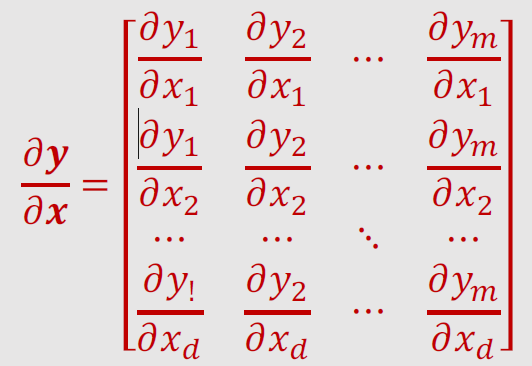
\includegraphics[width=0.8\linewidth]{images/jacobian_matrix.png}
                \caption{Structure of a Jacobian matrix for a vector function $y = f(x)$.}
            \end{figure}
        \end{column}
    \end{columns}
\end{frame}

\begin{frame}{From Scalars to Vectors}
    \framesubtitle{Vectorized Forward Pass}
    \begin{itemize}
        \item For a full layer $l$, we can compute the pre-activations $z^{[l]}$ for all neurons in that layer with a single matrix-vector multiplication:
        \[ z^{[l]} = W^{[l]}a^{[l-1]} + b^{[l]} \]
        \item Then, the activations $a^{[l]}$ are computed by applying the activation function $f$ element-wise to the vector $z^{[l]}$:
        \[ a^{[l]} = f(z^{[l]}) \]
    \end{itemize}
    \begin{figure}
        \centering
        % Source: MLP & Back-prop.pdf, Page: 63
        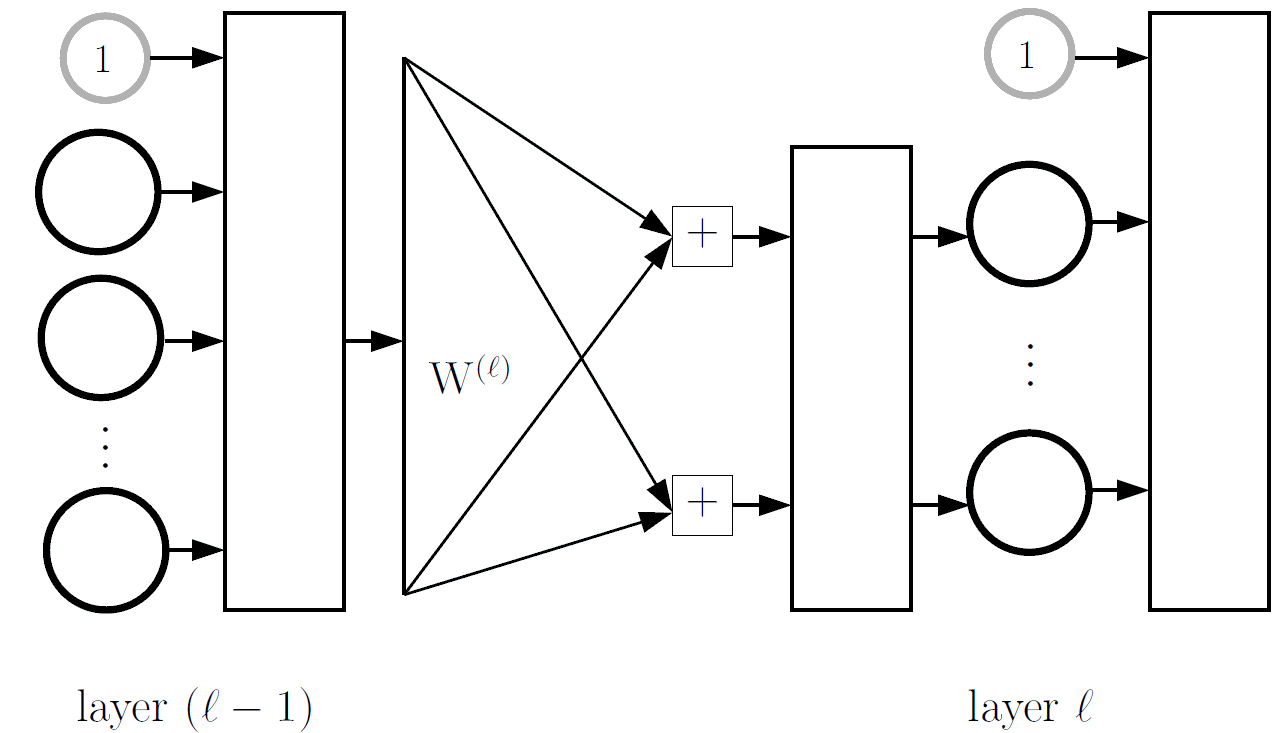
\includegraphics[width=0.7\linewidth]{images/vectorized_backprop.png}
        \caption{Vectorized data flow from the activations of the previous layer ($a^{[l-1]}$) to the current layer ($a^{[l]}$).}
    \end{figure}
\end{frame}

\begin{frame}{From Scalars to Vectors}
    \framesubtitle{Vectorized Backward Pass: The Sensitivity Vector}
    \begin{itemize}
        \item In the backward pass, our goal is to compute the gradient of the loss with respect to all parameters.
        \item The key quantity we propagate backward is the \bhighlight{sensitivity vector} (often called "error" or "delta"), defined as the gradient of the loss with respect to the pre-activation vector $z$ of a layer:
        \[ \delta^{[l]} = \frac{\partial \text{Loss}}{\partial z^{[l]}} \]
        \item This vector tells us how sensitive the final loss is to small changes in the input of the activation function for each neuron in layer $l$.
    \end{itemize}
\end{frame}

\begin{frame}{From Scalars to Vectors}
    \framesubtitle{Vectorized Backward Pass: The Chain Rule}
    \begin{itemize}
        \item We can compute the sensitivity of layer $l-1$ from the sensitivity of layer $l$ using the vectorized chain rule:
        \[ \delta^{[l-1]} = \frac{\partial z^{[l]}}{\partial a^{[l-1]}} \frac{\partial a^{[l-1]}}{\partial z^{[l-1]}} \frac{\partial \text{Loss}}{\partial z^{[l]}} \]
        \item This simplifies to a clean, efficient update rule:
        \[ \delta^{[l-1]} = (W^{[l]T}\delta^{[l]}) \odot f'(z^{[l-1]}) \]
        where $\odot$ is the element-wise product (Hadamard product). This formula is the core of backpropagation in practice.
    \end{itemize}
\end{frame}

\begin{frame}{From Scalars to Vectors}
    \framesubtitle{Vectorized Gradient Calculation}
    \begin{itemize}
        \item Once we have the sensitivity vector $\delta^{[l]}$ for a given layer, the gradients for the \emph{entire} weight matrix $W^{[l]}$ and bias vector $b^{[l]}$ of that layer can be computed with single vector operations:
        \[ \frac{\partial \text{Loss}}{\partial W^{[l]}} = \delta^{[l]}(a^{[l-1]})^{T} \]
        \[ \frac{\partial \text{Loss}}{\partial b^{[l]}} = \delta^{[l]} \]
        \item This vectorized approach is significantly more efficient than looping through individual weights and is the reason deep learning is computationally feasible today.
    \end{itemize}
\end{frame}